\chapter{Asking Billionaires How They Got RICH! (Boston)}

These notes follow the progression of a School of Hard Knocks interview set in Boston and curated for this book project by LazyingArt LLC. The lecture has no blackboard mathematics of its own, so we introduce a small amount of notation only where it helps us separate different kinds of quantity: annual income, company valuation, assets under management, cash runway, customer growth, and control rights. The central payoff is not a single formula for wealth, but a sequence of cases showing that product, courage, sales, discipline, and meaningful ambition do not enter the story in the same way.

\section{Boston as a Wealth Field}

The lecture opens theatrically. We are shown, in quick succession, an NBA star, a wearable-device founder, and a beer entrepreneur, and the montage ends with a warning: if the ambition is merely to become a billionaire, good luck. That warning is not an ornament. It is the first organizing principle of the chapter. We will spend the rest of the lecture discovering that the number itself is rarely the governing variable.

The host then reframes Boston as a field in which several wealth mechanisms coexist. It is not simply a rich city; it is a city in which athlete pay, startup valuation, hedge-fund scale, and founder-controlled product wealth can all be placed side by side. The first quantitative anchor is therefore demographic:

\begin{equation}
N_{\text{millionaires,Boston}} > 40{,}000,
\qquad
N_{\text{billionaires,Boston}} > 10.
\end{equation}

This already forces a small piece of bookkeeping on us. The lecture speaks freely about ``money,'' but the cases that follow involve very different objects. We will keep them separate:
\begin{itemize}
\item \(Y\): annual personal income or compensation,
\item \(V\): company valuation,
\item \(A\): assets under management,
\item \(W_t\): investable wealth evolving through time.
\end{itemize}

\begin{remark}
The lecture itself does not present these symbols. They are introduced here only to prevent a common confusion of categories. An athlete who earns \(Y\), a founder whose company is valued at \(V\), and an investor who helps oversee \(A\) are not being measured by the same thing.
\end{remark}

\section{Whoop: Problem First, Company Second}

The first full case is the founder of Whoop. The interview begins in the ordinary register of the series, with the question of when he became a millionaire, but it quickly shifts to the more interesting claim: he was not first trying to become an entrepreneur in the abstract. He was trying to solve a problem. He wanted to understand health and to build wearable devices that millions of people could use in order to improve their health. The company comes after the problem.

The basic scale markers are simple:

\begin{equation}
t_0 = 2012,
\qquad
T_{\text{build}} \approx 12\ \text{years},
\qquad
V_{\text{Whoop}} \approx \$3.6 \times 10^9.
\end{equation}

The important point is the order. The lecture does not say: first decide to start a company, then search for a market. It says, in effect: first find the problem that keeps hold of you, and only then let the company form around it.

\begin{definition}
A signal event is a public sign that is small in direct cash terms but large in informational value. It changes the founder's belief that the project may actually survive.
\end{definition}

The lecture gives a concrete instance of such a signal event in the Whoop story. In 2015, while the company was still struggling, the founder sees LeBron James wearing a Whoop device in a Kia commercial. At that moment the installed base is tiny:

\begin{equation}
N_{\text{Whoop straps at the LeBron moment}} \approx 100.
\end{equation}

That number matters because scarcity and elite adoption appear together. One device among roughly one hundred has reached the most visible athletic tier in the world. It is not yet a proof of business success, but it is a proof that the company is not imaginary.

\begin{figure}
\centering
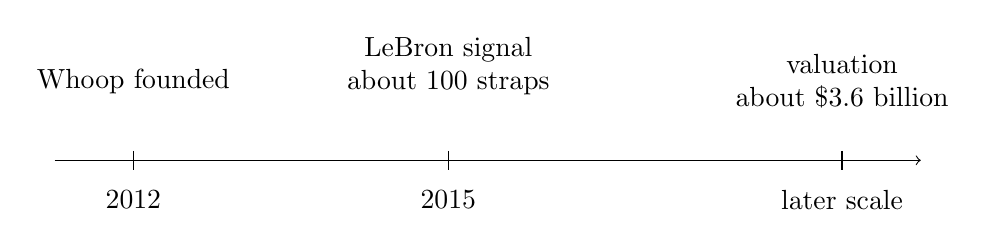
\begin{tikzpicture}[x=1cm,y=1cm]
\draw[->] (0,0) -- (11,0);
\draw (1,0.12) -- (1,-0.12);
\draw (5,0.12) -- (5,-0.12);
\draw (10,0.12) -- (10,-0.12);
\node at (1,-0.5) {2012};
\node at (5,-0.5) {2015};
\node at (10,-0.5) {later scale};
\node[align=center] at (1,1.0) {Whoop founded};
\node[align=center] at (5,1.2) {LeBron signal\\about \(100\) straps};
\node[align=center] at (10,1.0) {valuation\\about \(\$3.6\) billion};
\end{tikzpicture}
\end{figure}

The timeline matters because the lecture refuses a frictionless founder myth. Between founding and later scale there is a long middle in which the project is not yet self-justifying. The mathematics, thin as it is, is there only to keep that middle visible.

\section{Courage Under Liquidity Stress}

The strongest conceptual turn in the lecture comes when the host asks for a lesson not taught in business school. The answer is not vision, empathy, strategy, or even business acumen. It is courage. The reason is simple: when a company encounters a real problem, the difficulty is no longer abstract.

We can represent the founder's description of that pressure by a deliberately minimal schematic:
\begin{equation}
K_t \downarrow,
\qquad
P_t\ \text{due},
\qquad
q_t\ \text{uncertain}.
\end{equation}
Here \(K_t\) is available cash or runway, \(P_t\) is payroll and other immediate obligations, and \(q_t\) is the state of the product. The lecture names all three in ordinary language: almost running out of money, almost missing payroll, and a product that is failing.

\subsection{Question \& Answer}

\paragraph{Question.} What is the hardest trait in building a company when things are actually going wrong?

\paragraph{Answer.} The lecture's answer is courage. This is not courage in the theatrical sense, but in the managerial sense: saying the hard thing, doing the hard thing, and walking into the problem instead of trying to remain above it. Strategy is necessary, but strategy without the willingness to own the problem does not survive contact with a binding payroll date.

The sequence in the lecture is precise. We first hear that courage is the missing trait. Only after that do we hear the evidence: the company almost failed, and the founder was still broke six or seven years into the effort. The claim is therefore not motivational decoration. It is an attempt to explain what variable becomes decisive when the usual founder language stops helping.

\paragraph{Mechanism.} The LeBron moment enters here as a morale shock. It does not remove the equation
\[
K_t \downarrow,\qquad P_t\ \text{due},\qquad q_t\ \text{uncertain},
\]
but it changes the founder's internal estimate that the business may still be worth carrying. In that sense the signal event does not solve the firm; it keeps the founder from abandoning it.

\section{Product, Competition, and the Distribution Illusion}

Once the internal survival problem has been laid out, the lecture turns outward. Competition now appears, and the host asks the most natural question: what happens when a much larger company enters the same space? The answer is not that competition does not matter. The answer is that size and distribution are not the same thing as durable adoption.

Whoop is described as a product that is fully integrated, associated with a brand, and supported by strong data. The lecture's practical claim is that a mere copy is not the same as the object that users actually wear and love. We can compress that claim into a careful editorial shorthand:

\begin{align}
\text{large distribution} &\not\Rightarrow \text{durable adoption},\\
\text{better product} &\Rightarrow \text{repeat use and loyalty}.
\end{align}

The Amazon segment of the transcript is slightly rough, but the meaning is clear enough. A giant can manufacture distribution. It cannot automatically manufacture the specific collection of qualities that makes a product worth keeping on the body.

\subsection{Question \& Answer}

\paragraph{Question.} What beats large distribution: marketing power or a product that people actually love?

\paragraph{Answer.} The lecture answers in favor of the latter. Distribution matters, and the founder explicitly says that large competitors were taken seriously. But the operative variable is not size alone. It is whether the object contains the ``magic'' that keeps users attached to it. The lecture therefore resists two cheap slogans at once: it does not say that competition is irrelevant, and it does not say that scale always wins.

The section closes with a compressed founder blueprint. One finds something one loves, becomes obsessed with it, drops entitlement, works harder than others are willing to work, persists, builds a team, raises capital, and keeps going. It is worth noticing that the blueprint arrives only after the lecture has shown us near-failure and competition. In other words, the recipe is delivered only after the costs of the recipe have been made visible.

\section{Jalen Brown: Adversity, Social Capital, and Non-Desperation}

The Jalen Brown interview changes the grammar of wealth while keeping the money question alive. Here the central object is not company valuation but annual income:
\begin{equation}
Y_{\text{Brown,last year}} \approx \$5.0 \times 10^7.
\end{equation}

But the lecture refuses to let that quantity settle the issue. Brown says that adversity and failure are among the blessings in his life because they unlock work ethic, discipline, and creativity. The first move, then, is from success to adversity. The second move is from adversity to a theory of money. He says he does not keep a lot of money in the bank, and he adds that the richest people often do not, because money is ``just paper'' and because many of them are after social capital.

This is not a rigorous financial doctrine, and it should not be treated as one. But it is a serious distinction. A high \(Y\) does not tell us what the person values, how liquid the person remains, or whether the person approaches negotiation from need or from freedom. Brown insists that he can run away from a deal that does not align with him. Non-desperation, in the lecture, is itself a form of wealth.

The section deepens again. Brown speaks about growing up without money, providing for his family, dealing with hatred in public life, and then offers the lecture's most memorable metaphor: the moon steals light from the sun, but people do not confuse the two. It is a way of speaking about imitation without insecurity. The true source remains the source.

From there the lecture descends into doubt, anxiety, depression, and faith. This descent matters. It tells us that a public measure like \(Y_{\text{Brown}}\) is a radically incomplete description. The lecture wants us to see that wealth, performance, and visibility do not remove darkness; at most they alter its setting. The final answer is neither technical nor economic. It is faith, consistency, and hard work.

\paragraph{A short interlude on writing.} Before the next interview, the host inserts a brief practical aside: many opportunities begin with an email, and writing is part of how one pitches, leads, hires, and connects. This interlude should not carry the chapter, but it does preserve the lecture's rhythm. After public success and interior struggle, the talk briefly returns to technique at the level of communication.

\section{The Hedge-Fund Operator: Indexing, Giving, and the Household Decision}

The next interview introduces a different scale entirely:
\begin{equation}
A_{\text{managed}} \approx \$4.0 \times 10^{10}.
\end{equation}
Here we are no longer dealing with startup valuation or athlete income, but with institutional capital. The speaker reports roughly twenty-one years at a hedge fund, senior-partner status, and management at the level of about forty billion dollars. Yet the advice immediately turns downward, away from institutional complexity and toward ordinary discipline.

\subsection{Question \& Answer}

\paragraph{Question.} Where should most people put their money if they know less than they think they know?

\paragraph{Answer.} The lecture's answer is disarmingly plain: an index fund, and specifically the S\&P 500 through a low-cost provider such as Vanguard. The underlying principle is epistemic modesty. Smart people know what they know and what they do not know. The lecture therefore treats simplicity not as lack of sophistication, but as the correct response to uncertainty.

To make that advice mathematically useful, we can write the standard compounding recurrence
\begin{align}
W_{t+1} &= (1+r)W_t + s_t,\\
W_0 &= 0,
\end{align}
where \(W_t\) is investable wealth at time \(t\), \(r\) is the period return of the chosen broad market vehicle, and \(s_t\) is the contribution added during the period. This is not a lecture formula; it is a clean reconstruction of the compounding logic the interview gestures toward.

Let us work out the simplest constant-savings example. Suppose \(s_t=s\) each period. Then
\begin{align}
W_1 &= s,\\
W_2 &= (1+r)s + s,\\
W_3 &= (1+r)^2s + (1+r)s + s.
\end{align}
Continuing in this way, we obtain
\begin{equation}
W_n = s\sum_{k=0}^{n-1}(1+r)^k
    = s\,\frac{(1+r)^n-1}{r}.
\end{equation}
This is the mathematical heart of the interview's practical advice. One need not discover a secret stock. One must repeatedly contribute to a broad vehicle and allow time to do the multiplying.

But the lecture again refuses to end with a financial formula. When asked about the largest amount of money made in a single year, the speaker redirects the question toward how much was given away. When asked whether money buys happiness, the answer is no: money makes one more of what one already is. Then come faith and mortality. By the time the lecture reaches marriage, the best financial decision is no longer an asset purchase at all, but the choice of a life partner whose character is aligned with one's own work and commitments.

The final ethical formula in this section is verbal rather than algebraic: self-interest is essential, selfishness is not. That distinction belongs here because the lecture wants household finance and moral judgment to appear in the same frame.

\section{Jim Cook: Selling, Scarcity, and Control}

The Samuel Adams interview is the lecture's fullest founder case after Whoop, and it proceeds by overturning one expectation after another. A beer company that looks iconic from the outside is described, from the inside, not as a triumph of branding but as a triumph of product and sales effort.

The transcript provides several useful markers:
\begin{equation}
\Delta t_{\text{launch}\to\text{best beer}} \approx 6\ \text{weeks},
\qquad
T_{\text{first marketing hire}} \approx 10\ \text{years},
\qquad
N_{\text{salespeople at that point}} = 80.
\end{equation}
These numbers do real work. If the first marketing hire arrives only after about a decade, and by that point there are already eighty salespeople, then the lecture is not merely making a rhetorical distinction between marketing and selling. It is describing an actual allocation of effort.

The naming story sharpens the point. Two names tested roughly equally well. Therefore the founder does not treat naming as the decisive explanatory variable. A better glass of beer matters more than the surface layer of branding. The principle is blunt: marketing is overrated; selling is underrated.

The most life-changing conversation in the section comes from the founder's uncle. Jim spends his day shopping for computers and trying to save small amounts of money, and the uncle cuts through the logic immediately: many businesses have gone broke with computers; they went broke because they had no sales. This is where the lecture becomes almost algorithmic:
\begin{equation}
N_{t+1}=N_t+1.
\end{equation}
The formula is deliberately crude. It represents the instruction to get one customer every day and not come home until that customer exists. It is not intended as a realistic growth law for a mature enterprise. It is a discipline rule for a young founder.

If we begin at \(N_0=0\), then after \(30\) days of genuine execution the rule says
\[
N_{30}=30.
\]
The point is not the exact number. The point is that business motion is being generated by contact with customers rather than by endless preparation.

The shoestring logic of the company is equally concrete. The founder does not build a brewery; he contracts production. He does not pay for an office; he uses bars and pay phones. He spends on what cannot be faked: ingredients, brewing excellence, and market entry. When cash cannot purchase the best brewmaster in the world, equity does the work:
\begin{equation}
e_{\text{brewmaster}} = 0.02.
\end{equation}
This is a clean case of substituting ownership for cash compensation when expertise is indispensable and liquidity is scarce.

The same economy appears in the later question of public markets and control:
\begin{equation}
t_{\text{public}} = 1995.
\end{equation}
The lecture's notable claim is that going public need not mean surrendering control. The founder says, in effect, that he sacrificed some economics in order to keep the voting shares. As a schematic, one may write
\begin{equation}
C \uparrow \quad \Longrightarrow \quad E \downarrow \ \text{may be accepted},
\end{equation}
where \(C\) denotes control rights and \(E\) the purely economic claim. This again is an editorial shorthand rather than a lecture formula, but it captures the stated tradeoff.

The section closes by returning us to the opening warning of the chapter. If the ambition is merely to become a billionaire, good luck. If the ambition is to make great beer and launch a beer revolution, then one may do very well. Wealth, the founder says, is in some sense life's booby prize. Happiness is the better terminal variable.

\section{Summary}

Boston, in this lecture, is less a city than a comparison device. We pass from athlete income to startup valuation, from hedge-fund scale to founder-controlled product wealth, and the lecture repeatedly insists that we not mistake one for another. The few formulas we have written are therefore sorting devices before they are anything else.

What remains after the sorting is a compact doctrine. Problem-first entrepreneurship matters more than entrepreneurial self-image. Courage becomes decisive when cash is tight and the product is still uncertain. Distribution without a product people love is fragile. For ordinary investing, compounding in a broad index fund is better than unnecessary cleverness. In company building, product and sales beat branding theater, and control may be worth sacrificing economics for. Above all, the lecture does not permit wealth to stand alone as a goal. Meaningful ambition, character, and the uses to which money is put remain the larger frame in which all of the smaller quantities must finally be read.